\documentclass[11pt,parskip]{scrartcl}
\usepackage[ngerman]{babel}

% For XeTeX %%%%%%%%%%%%%%%%%%%%%%%%%%%%%%%%%%%%%%%%%%%%%%%%%%%%%%%%%%%%%%%%%%%%
\usepackage{fontspec}
\setromanfont{Linux Libertine O}
\setsansfont{Linux Biolinum O}

% For pdfTeX %%%%%%%%%%%%%%%%%%%%%%%%%%%%%%%%%%%%%%%%%%%%%%%%%%%%%%%%%%%%%%%%%%%
%\usepackage[T1]{fontenc}
%\usepackage{inputenc}
%\usepackage{mathpazo}

% Packages %%%%%%%%%%%%%%%%%%%%%%%%%%%%%%%%%%%%%%%%%%%%%%%%%%%%%%%%%%%%%%%%%%%%%
%\usepackage{biblatex}
\usepackage{amsmath}
\usepackage[a4paper]{geometry}
\usepackage{graphicx}
\usepackage{xcolor}
\usepackage{microtype}
\usepackage{booktabs}
\usepackage[colorlinks=false, pdfborder={0 0 0 }]{hyperref}
\usepackage{cleveref}
\usepackage[autostyle=true,german=quotes]{csquotes}
\usepackage{blindtext}
%\usepackage{listings}
\usepackage{tcolorbox}
\tcbuselibrary{listings}
\usepackage{siunitx}

% Options %%%%%%%%%%%%%%%%%%%%%%%%%%%%%%%%%%%%%%%%%%%%%%%%%%%%%%%%%%%%%%%%%%%%%%
\widowpenalty=10000
\clubpenalty=10000

\definecolor{light-gray}{gray}{0.95}
\tcbset{
    listing only,
    colback=light-gray,
    coltext=black,
    boxrule=0pt,
    left=-2.5pt
  }


% Begin of document %%%%%%%%%%%%%%%%%%%%%%%%%%%%%%%%%%%%%%%%%%%%%%%%%%%%%%%%%%%%
\begin{document}


% Titlepage %%%%%%%%%%%%%%%%%%%%%%%%%%%%%%%%%%%%%%%%%%%%%%%%%%%%%%%%%%%%%%%%%%%%
%
\begin{titlepage}
  \begin{sffamily}
    {\scshape\LARGE \textcolor{gray}{Universität Hamburg}\par}
    {\scshape\Large \textcolor{gray}{Projektarbeit Interactive Visual
        Computing}\par}
    \vspace{2.5cm}
    \centering
    {\huge\bfseries Es war einmal ein Babytux\ldots\par}
    {\large\bfseries Ein Povray-Animationsfilm\par}
    \vspace{1.5cm}
    {\Large\itshape \textcolor{darkgray}{
        Lemme, Inga \quad{}
        Ort, Thomas \quad{}
        Remmels, Melanie
      }\par
    }
    \vfill
    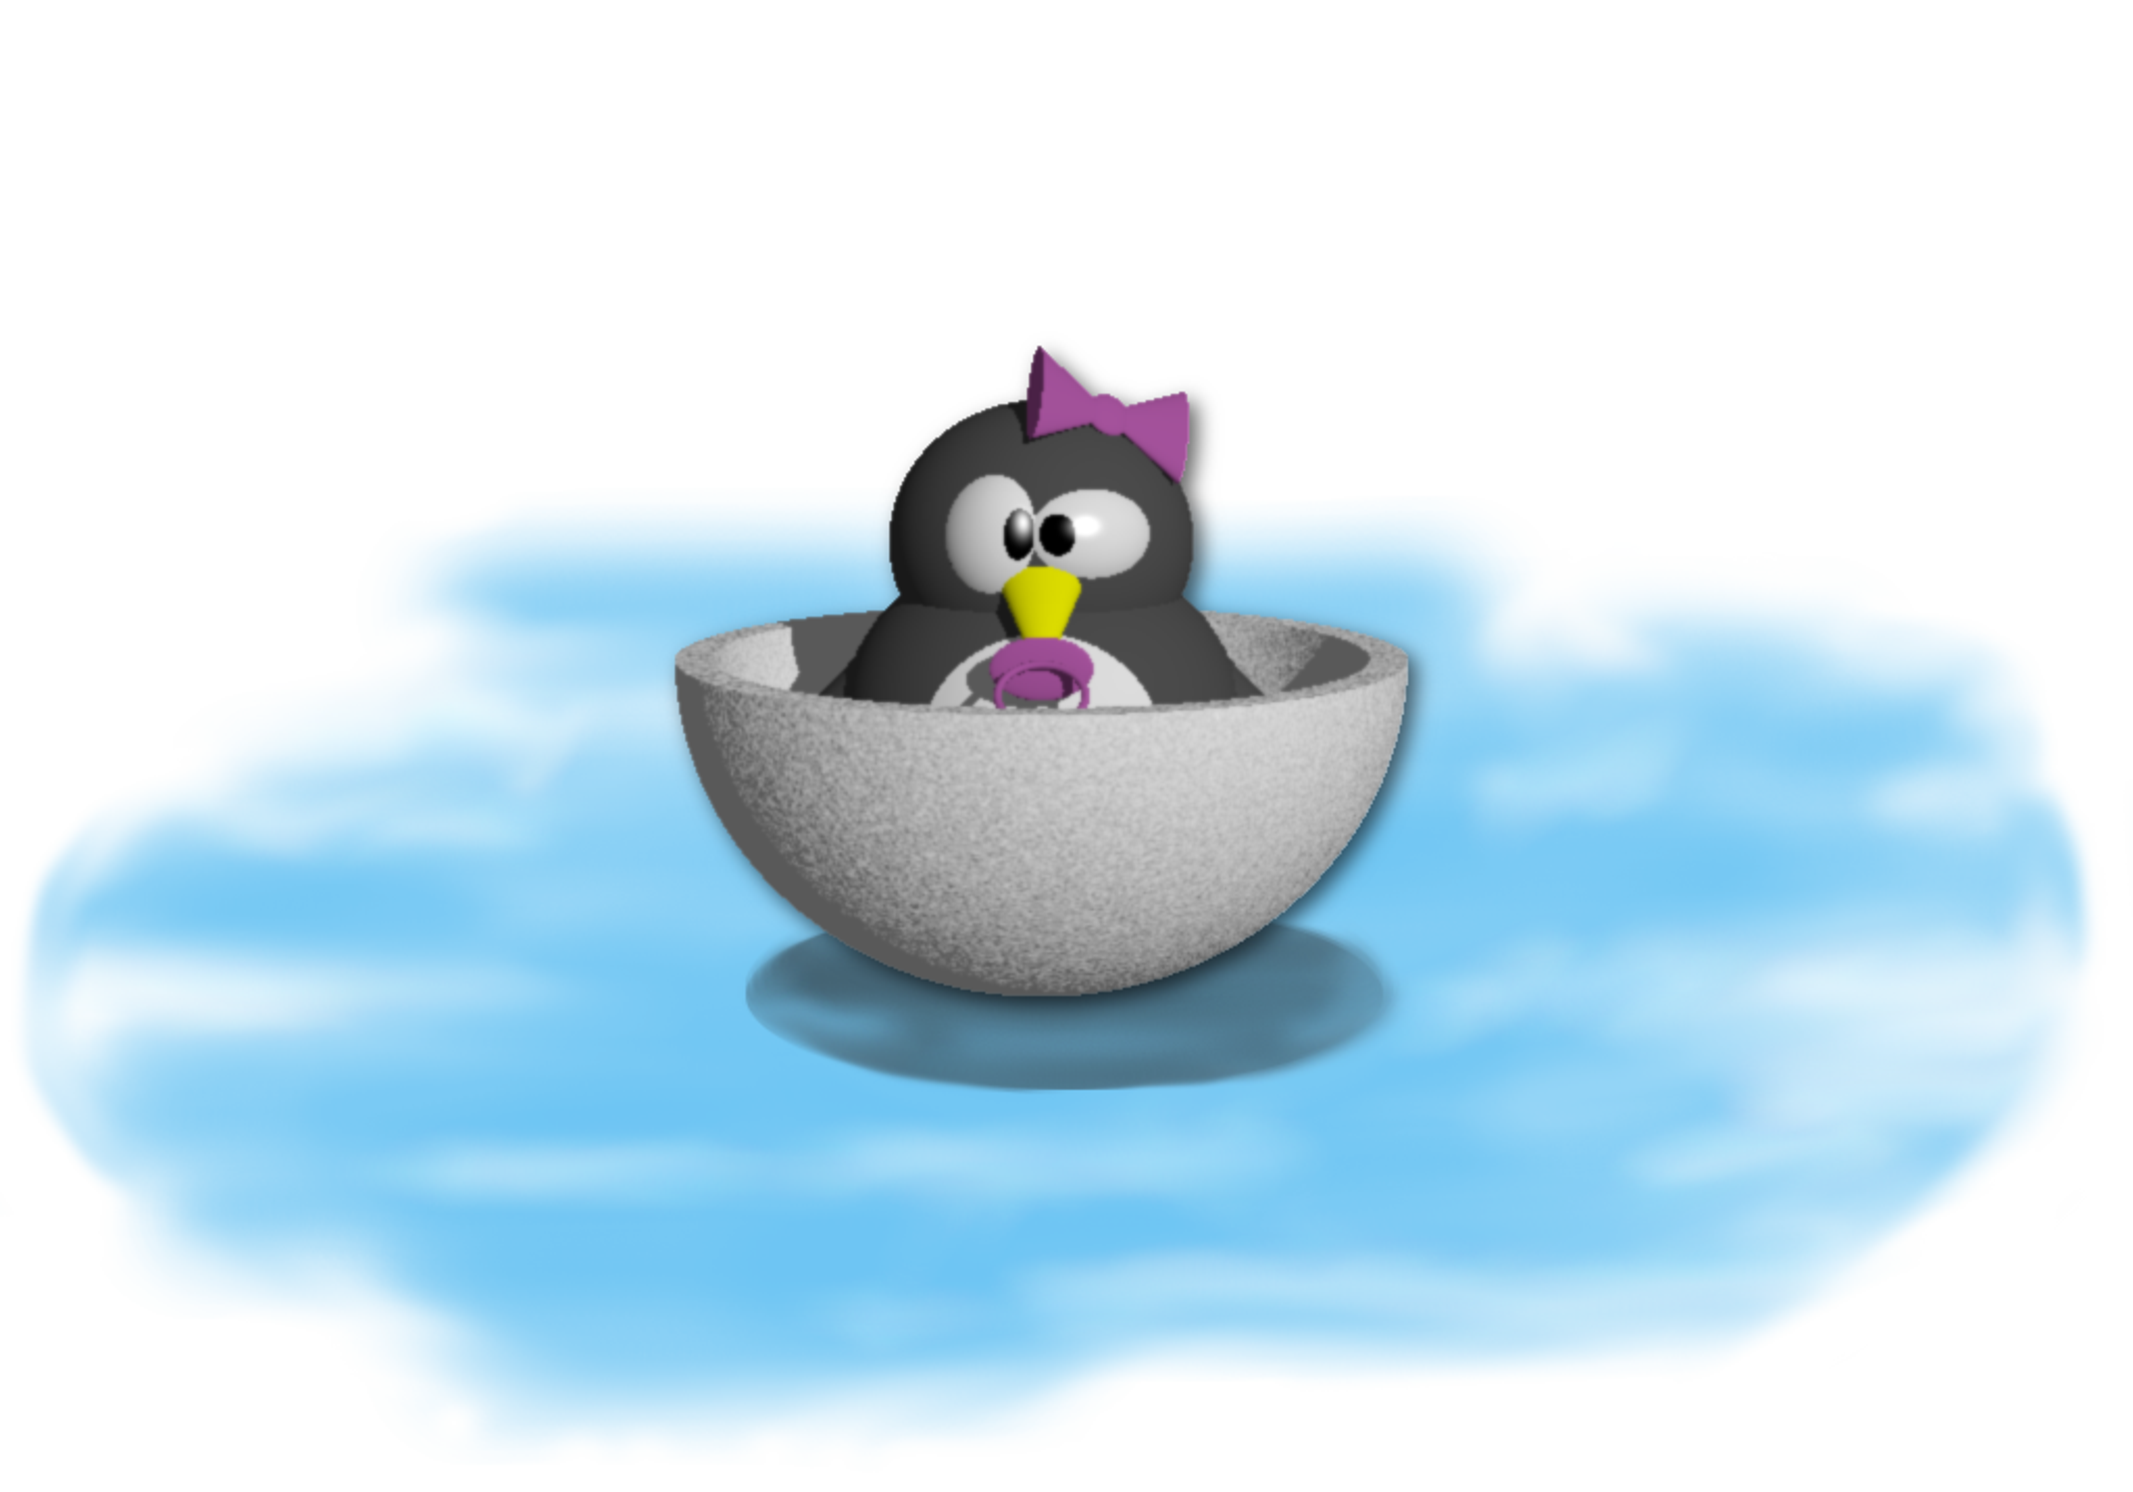
\includegraphics[width=0.75\textwidth]{./fig/ourtux4.pdf}\par\vspace{1cm}
    \vfill
    % Bottom of the page
    {\large \today\par}
  \end{sffamily}
\end{titlepage}
%
% End of Titlepage %%%%%%%%%%%%%%%%%%%%%%%%%%%%%%%%%%%%%%%%%%%%%%%%%%%%%%%%%%%%%


\newpage
\tableofcontents
\newpage


\section{Projektidee}
Vorlage für die Hauptfigur des hier beschriebenen Films wurde das Maskottchen des
freien Kernels \emph{Linux}. Dieses stellt einen Pinguin dar und wird kurz
\emph{Tux} genannt. \emph{Tux} wurde im Jahr 1996 von \emph{Larry Ewing} mit
der Bildbearbeitungssoftware \emph{GIMP} entworfen und steht seitdem zur freien
Verfügung für die Gemeinde. Er darf nach Belieben verwendet und verändert
wurden, solange auf Nachfrage sowohl Urheber\footnote{lewing@isc.tamu.edu} als
auch das verwendete Programm genannt wurden. \cite{ewing}

Die Idee, dass das Logo ausgerechnet einem Pinguin nachempfunden wurde, stammt
von \emph{Linus Torvalds}, dem Gründer von Linux. Laut \emph{Jeff Ayers}, einem
Linuxentwickler, besitzt \emph{Torvalds} eine Affinität für
\enquote{\emph{flugunfähige, fette Wasservögel}}, sodass letztlich der Entwurf
von \emph{Ewing} übernommen wurde. Eine weitere Anekdote, die zur Auswahl des
Pinguins beigetragen hat stammt von einem Erlebnis \emph{Torvalds} in einem
Aquarium in Canberra, Australien. Dort wurde er von einem Pinguin gebissen und
sei seitdem mit der Krankheit \emph{Penguinitis} infiziert:

\begin{quote}
  \enquote{Penguinitis makes you stay awake at nights just thinking about
    penguins and feeling great love towards them.} \cite{tuxstory}
\end{quote}

Es gibt inzwischen unzählige Versionen des Maskottchens, in dieser
Arbeitsgruppe haben wir uns an einer modernen und jungen Version des Pinguins
orientiert wie in Abbildung \ref{fig:overlord59tux} zu sehen.

\begin{figure}[htbp]
  \centering
  
\includegraphics[width=0.3\textwidth]{./fig/overlord59tux.pdf}
  \caption{
    Die Hauptfigur des Filmes wurde nach diesem Vorbild entwickelt. Das
    gezeigte Modell stammt vom Autor \emph{Overlord59} und wurde unter
    \emph{Creative Commons BY-NC-SA} veröffentlicht.
    \emph{
      (Quelle:
      \url{http://tux.crystalxp.net/de
        .id.1568-overlord59-overlord59-tux-g2.html)
      }
    }
  }
  \label{fig:overlord59tux}
\end{figure}


\subsection{Plot des Films}
Zu Beginn des Films wurde zunächst ein Ei zu sehen, welches immer größere Risse
bekommt und anschließend ein Stück aus dem Ei heraus bricht. Aus dem
heraus gebrochenen Stück schauen die Augen des Tux.

Der obere Teil des Eis bricht auf und letztlich schlüpft der Tux. Anschließend
entdeckt der Pinguin, dass er Füße, Flügel und seinen Schwanz bewegen kann.
Nachdem er sich etwas umsieht beginnt er seine Gegend zu erkunden und läuft
los.

Im weiteren Verlauf wird ein Zeitraffer-Effekt eingesetzt. Der Tux wächst
langsam und entdeckt dabei die schönen und schwierigen Dinge des Lebens.

\subsection{Liste der Povray-Module}

Im Folgenden sind alle Module beschrieben, die im Projekt erstellt und verwendet
wurden.

\begin{description}
  \item [environment.pov] Aufbau der Umgebung; enthält Himmel und Boden.
  \item [egg.pov] Geschlossenes Ei-Objekt.
  \item [tux.pov] Körper des Tux ohne Accessoires.
  \item [bow.pov] Pinke Schleife.
  \item [soother.pov] Schnuller.
  \item [assempledTux.pov] Zusammengebauter Tux mit Accessoires.
  \item [crack.pov] Objekt zum Erstellen eines Risses im Ei-Objekt.
  \item [tuxIsBorn.pov] Animation des wackelnden Eis und Animation der
    Risse; Tux erscheint im Ei mit animiertem Nuckeln am Schnuller.
  \item [babytuxDiscovers.pov] Animation der beweglichen Gliedmaßen des Tux.
\end{description}

\newpage

\section{Statischer Aufbau der Figuren}
Im Folgenden wird beschrieben mittels welcher povray-Funktionen und Objekte die
einzelnen Figuren, Requisiten und Szenenbilder des Films erstellt wurden.


\subsection{Konstruktion der Umgebung}
In der Datei \texttt{environment.pov} wurden alle relevanten Objekte der Umgebung
festgelegt. Der Himmel wurde mittels \texttt{sphere} der Boden mittels
\texttt{plane} realisiert. Dabei wurde für den Himmel eine \texttt{color\_map}
eingesetzt um einen Farbverlauf herzustellen. Für eine unebene Struktur des
Bodens wurde das Pattern \texttt{bumps} verwendet.


\subsection{Aufbau des Pinguineis}
Die Grundstruktur des Eis wurde von der Vorgängergruppe (Teil 1) übernommen
und an unseren Film angepasst. Dazu wurden jeweils für den oberen Teil und den
unteren Teil des Eis ein weiteres etwas kleineres Ei-Objekt erzeugt und mittels
\texttt{difference} vom größeren Objekt abgezogen. Dadurch wird das Ei von
innen hohl. Damit das jeweilige Objekt auch als hohl erkannt wird, wurde das
innere Objekt minimal nach oben bzw. nach unten verschoben.
%
\begin{tcblisting}{}
    difference{
    object{ Egg_lowerpart }
    object{
      Egg_lowerpart
      translate <0, 0.1, 0>
      scale <0.9, 0.9, 0.9>
    }
  }
\end{tcblisting}


\subsection{Aufbau der Hauptfigur}

\subsubsection{Körper}
Zu allererst wurden die Proportionen als \texttt{declare}-Anweisung festgelegt.
Um die Proportionen unabhängig von der Größe des Tux gleich zu halten, wird
nur die Höhe \texttt{tuxheight} variabel gehalten. Die anderen Größen wie
\texttt{tuxwidth} oder \texttt{radiustummy} wurden mit \texttt{tuxheight}
verrechnet.

Der Grundaufbau des Tux besteht aus zwei Grundkugeln, in povray \texttt{sphere}
genannt. Einer unteren großen Kugel für den Unterleib und einer etwas kleineren
Kugel für den Kopf oberhalb. Der Unterleib besteht zunächst aus \emph{einer}
Kugel. Zur Realisierung des weißen Bauches exwurdeieren zwei weitere
\texttt{sphere}-Objekte, deren Schnittmenge (\emph{intersection}) anschließend
mit der großen Kugel vereinigt wird (\emph{union}).
%
\begin{tcblisting}{}
  union{
    intersection{
      sphere{ 0, radiustummy }
      sphere{ 0, radiustummy }
      scale <0.6, 1.5, 0.25>
      translate <0, 0, -radiustummy + 0.1>
    }
    pigment{ White }
    sphere{
      0, radiustummy
      pigment{ Gray10 }
    }
  }
\end{tcblisting}
%
Die weiße Schnittmenge wurde mit den Funktionen \texttt{scale} und
\texttt{translate} so verschoben und skaliert, dass der vordere Teil der
Hauptkugel in den richtigen Proportionen weiß erscheint. Sowohl Kopf, als auch
Unterleib wurden in einer \texttt{declare}-Anweisung als \texttt{head} und
\texttt{tummy} global geltend gemacht. So können diese direkt angesprochen
wurden, ohne den Code immer wieder neu reproduzieren zu müssen.

Der Kopf des Pinguins wurde mit einer \texttt{sphere} generiert, die zwei Drittel
der Größe des Unterleibes beträgt. In den Kopf wurden Augen mit schwarzen Pupillen
eingelassen. Zunächst wurde die Pupille in einer \texttt{declare}-Anweisung
festgelegt. Sie besteht wie der Bauch aus der Schnittmenge zweier Kugeln. Die
beiden Augen wurden in \texttt{LeftEye} und \texttt{RightEye} deklariert. Hier
wurden die Pupillen als Objekt mit einem weiteren \texttt{sphere}-Objekt
vereinigt (\texttt{union}).

Der Schnabel des Tux wurde mittels eines \texttt{cone}-Objektes realisiert.
Hierbei wurden Zentrum und Radius der beiden Enden, sowie die Skalierung des
gesamten Objektes so gewählt, dass ein flach gedrückter Kegel entsteht.

\subsubsection{Gliedmaßen}
Der Tux besteht weiterhin aus zwei Füßen und zwei Flügeln. Die Flügel bestehen
aus jeweils einem Objekt \texttt{Wing}, welches aus einer Differenz aus
\texttt{cone} und \texttt{sphere} gebildet wurde. Die Füße bestehen aus dem
Objekt \texttt{Foot}, der Schnittmenge aus \texttt{sphere} und \texttt{box}.
Dadurch wurde die Sphäre halbiert und es ist nur die obere Hälfte sichtbar.

In der Rückansicht ist ein Schwanz zu sehen. Dieser wurde aus einer einfachen
\texttt{cone} in passender Größe generiert und lässt sich als
\texttt{Tail}-Objekt ansprechen.

\subsubsection{Accessoires}
Der Tux ist in diesem Film ein weibliches Jungtier, daher wurde eine Schleife
(\texttt{Bow}) und ein Schnuller (\texttt{Soother}) konstruiert. Die Schleife
wurde zunächst als ein \texttt{PartBow}-Objekt deklariert, welches eine
\texttt{cone} generiert. In einer \texttt{union} wurden anschließend zwei dieser
Objekte zusammengefügt, wobei eines um \ang{180} gedreht wurde. Der Knoten der
Schleife wurde innerhalb der \texttt{union} mittels \texttt{sphere} umgesetzt.

Für den Schnuller wurde eine \texttt{sphere} und ein \texttt{torus} vereinigt.
Die beiden Accessoires wurden in jeweils eine Datei ausgelagert, dadurch sind
die Objekte vom eigentlichen Körper unabhängig und können bei Bedarf auch
weggelassen werden.


\subsection{Bewegliche Gliedmaßen}
\newpage


\section{Aufbau der einzelnen Animationssequenzen}
Der überwiegende Teil der einzelnen Sequenzen wurde jeweils innerhalb einer
Datei mittels der Funktion \texttt{clock} und mehreren \texttt{if}-Schleifen
realisiert. Dazu wurde zu Beginn die Variable \texttt{MyClock} deklariert.

Bsp.:
%
\begin{tcblisting}{}
  #declare My_Clock = Start + (End - Start) * clock;

  #if (My_Clock <= 1)
  /* tue etwas */

  #elseif(My_Clock <=2)
  /* tue etwas anderes */
  ...
\end{tcblisting}
%
Mittels dieser Deklarationen war es möglich die folgenden kurzen Sequenzen zu
erstellen.

\subsection{Titelsequenz}

\subsection{Sequenz 1: Erstes Anzeichen von Leben}
Das Ei beginnt sich mehrere Male hin und her zu bewegen. Dazwischen gibt es
immer wieder Pausen. Dazu wurde die sinus-Funktion verwendet. Dabei werden

\subsection{Sequenz 2: Schlüpfen des Tux}
Zunächst bekommt das Ei einen Riss, welcher immer größer wird und sich um das
ganze Ei ausdehnt. Sobald die obere Hälfte von der Unteren des Eis komplett
getrennt ist, hebt die obere Hälfte ab und fliegt nach hinten weg.

Zur Realisierung dieser Szene wurde ein Objekt \texttt{Crack} erstellt.
\texttt{Crack} besteht aus mehreren quadratischen \texttt{box}-Objekten die
ineinander verdreht wurden.
%
\begin{tcblisting}{}
  union{
    box{
      <-0.5, 0, -0.5>
      <0.5, 0.1, 0.5>
    }
    box{
      <-0.5, 0, -0.5>
      <0.5, 0.1, 0.5>
      rotate <5, 20, 10>
    }
    ...
  }
\end{tcblisting}
%
Dieses Objekt wurde so klein erstellt, dass es in das Ei-Objekt passt.
Anschließend wurde das \texttt{crack}-Objekt abhängig von der Zeit in der x- und
z-Richtung größer skaliert und eine Differenz zum Ei-Objekt gebildet. Die
Animation zeigt im Ergebnis einen Riss, der sich immer mehr vergrößert und am
Ende zwei Ei-Hälften erscheinen.

\subsection{Sequenz 2: Babytux entdeckt seine beweglichen Gliedmaßen}


\subsection{Sequenz 3: Babytux macht erste Gehversuche}


\subsection{Abschlusssequenz}
In der Abschlusssequenz erscheint der Originaltux von Larry Ewing als
Grafik\ldots

\newpage


\section{Fertigstellung des gesamten Films}


\subsection{Zusammenfügen der einzelnen Sequenzen}


\subsection{Vertonung}


\subsection{Korrekturen}


\newpage
\addcontentsline{toc}{section}{Literatur}
\bibliographystyle{unsrt}
\bibliography{bibtux}

\end{document}
